\documentclass[aps,physrev,10pt,floatfix,longbibliography,nofootinbib,reprint]{revtex4-2}

\usepackage{graphicx}% Include figure files
\usepackage{dcolumn}% Align table columns on decimal point
\usepackage{bm}% bold math
\usepackage{hyperref}% add hypertext capabilities
\usepackage[mathlines]{lineno}% Enable numbering of text and display math
%\linenumbers\relax % Commence numbering lines

\usepackage[%Uncomment any one of the following lines to test 
scale=0.7, marginratio={1:1, 2:3}, ignoreall,% default settings
text={7in,10in},centering,
%%margin=1.5in,
%%total={6.5in,8.75in}, top=1.2in, left=0.9in, includefoot,
%%height=10in,a5paper,hmargin={3cm,0.8in},
]{geometry}
\usepackage[utf8]{inputenc}
\usepackage{amsmath}
\usepackage{amstext}
\usepackage{graphicx}
\usepackage{esint}
\usepackage{geometry}
\usepackage{hyperref}
\usepackage{amsfonts}

\hypersetup{
    colorlinks=true,
    linkcolor=blue,
    filecolor=magenta,      
    urlcolor=cyan,
    pdftitle={Overleaf Example},
    pdfpagemode=FullScreen,
    }
%\geometry{verbose,lmargin=2cm,rmargin=2cm}

\begin{document}

\title{Autoregressive neural network of spins system: the deepness of Mean-Field models}
\author{Biazzo, Indaco}
 \altaffiliation[Also at ]{Physics Department, XYZ University.}%Lines break automatically or can be forced with \\

\date{\today}

\begin{abstract}
    An article usually includes an abstract, a concise summary of the work
    covered at length in the main body of the article. 
    \begin{description}
    \item[Usage]
    Secondary publications and information retrieval purposes.
    \item[Structure]
    You may use the \texttt{description} environment to structure your abstract;
    use the optional argument of the \verb+\item+ command to give the category of each item. 
    \end{description}
    \end{abstract}
    
    %\keywords{Suggested keywords}%Use showkeys class option if keyword
                                  %display desired
    
\maketitle

\tableofcontents

\section{Introduction}

1. Both Statistical physics and Machine learning deal with high dimensional input functions.\\
2. In the last years the generative power on new neural network frameworks achieve astonish results in many different domains.\\
3. The connections between statistical physics and Machine learning are a lots during last years, producing important and fundamental results in both domains. FOr instance applications of ML technics in statistical physics range from quantum mechanics, to classical stastical physics to chemical physics and complex systems. On the other way around applications of statistical physics concept have be used to understand the ability of SGD algorithms to explore the space of parameters of the neural network during the training, or the generalization capability, and to develop new architecture (cite stable diffusion).\\
4. In particular when we consider generative model, the autoregressive neural network connections become more close. Describe what are the autoregressive models, and what they allow and how are they used in statistical physics. Usually in statistical physics community the Machine learning architecture has been used. But the knowing of the model we want to sample from could be used to better shape the depp architecture of neural net. Moreover could be usefull to better understand why some architecture work better than other and in the end sheld light to the usual called black box of neural network underground model.\\
5.In this work concentrate on classical spins systems with pairwise interacting hamiltonian.For those systems in this work is shown how to derive autoregressive neural network architecture directly from the hamiltonian, where all the parameters of the neural network are directly related to the hamiltonian parameters.\\
6. In general the ANN architectures for these systems involve a exponentially growing with the number of spins in  systems. We derive for two mean field model, namely the Curie-Weiss model and the Sherrington-Kirkpatrick model, a new architecture where the number of params scale polinomially with N.\\
7. Several interesting future can be derived that this derived architecture shared with common used architecture:
      a. The solutions founded are deep.
      b. They have residual connections.
      c. They have skip connections (?).
      d. they are recurrent by construction.
      e. They are able to learn the hamiltonian parameters (?) [check].
      f. teh first layer parameters are related to the hamiltonian parameters, and they are shared.

      In this paper, we explore the connections between Statistical Physics and Machine Learning, specifically in the context of generative models. Both fields deal with high-dimensional input functions. In recent years, using neural network-based frameworks in Machine Learning has achieved remarkable success in various domains. The overlap between these fields has led to fundamental results, with applications of Machine Learning techniques in Statistical Physics spanning a wide range of areas, including quantum mechanics, classical statistical physics, chemical physics, and complex systems.

      On the other hand, applying concepts from Statistical Physics has been used to shed light on the behavior of Machine Learning algorithms. For example, understanding how the space of parameters of a neural network is explored during training, or how well the model generalizes to new data can be aided by looking at the problem through the lens of statistical physics. Additionally, the application of statistical physics concepts can lead to the development of new neural network architectures.
      
      In this work, we focus on classical spin systems with pairwise interacting Hamiltonians. These systems are commonly studied in statistical physics, and our goal is to show how to derive autoregressive neural network architectures directly from the Hamiltonian of these systems. Autoregressive models are a type of generative model that predict the next element in a sequence given all previous elements. In our case, the sequence is the configuration of spins in the system, and the goal of the model is to learn to generate new configurations that are likely according to the Hamiltonian. By deriving the neural network architecture from the Hamiltonian, we can establish a direct link between the parameters of the Hamiltonian and the parameters of the neural network.
      
      In general, ANN architectures for these systems tend to involve an exponential growth in the number of parameters with the number of spins in the system. However, we derive new architectures for two mean-field models, namely the Curie-Weiss model and the Sherrington-Kirkpatrick model, where the number of parameters scales polynomially with the number of spins. This is a significant improvement, as it allows for the scalability of the model to large systems. Our derived architecture also shares several interesting properties with commonly used architectures, such as being deep, having residual and skip connections, being recurrent by construction, and being able to learn the Hamiltonian parameters. Additionally, the parameters of the first layer of the network are directly related to the Hamiltonian parameters and are shared among all the spins, which allows to take advantage of the underlying symmetry of the problem to learn more efficiently.
            

%\section{Materials and Methods}
\section{Pair-wise Ising model in autoregressive conditional probability form}
Consider a generic Hamiltonian $H[\mathbf{x}]$ that depends on a set of $N$ binary variables $\mathbf{x}=\{x_1, x_2,...x_N\}$. The Boltzmann distribution at inverse temperature $\beta$ is:
\begin{equation}
P\left(\mathbf{x}\right)=\frac{e^{-\beta H\left(\mathbf{x}\right)}}{\sum_{\left\{ x\right\} }e^{-\beta H\left(\mathbf{x}\right)}}.
\end{equation}
It is generally challenging to compute marginals and average quantities when $N$ is large, and sampling from these distributions is difficult on frustrated systems. I defined the sets of variables $\mathbf{x}_{<i}=\left(x_{1},x_{2}\dots x_{i-1}\right)$ and $\mathbf{x}_{>i}=\left(x_{i+1},x_{i+2}\dots x_{N}\right)$ respectively with an index lower and larger than $i$, then if we can rewrite the Boltzmann distribution in the autoregressive form:
\begin{equation}
P\left(\mathbf{x}\right)=\prod_{i}P\left(x_{i}|\mathbf{x}_{<i}\right)
\end{equation}
then it would be straightforward to produce independent samples from it, thanks to the ancestral sampling procedure. It has been proposed to use a variational approach to approximate the Boltzmann distribution with trial probability distributions that have this autoregressive form where each conditional probability is represented by a feed-forward neural network with a set of parameters ${\theta}$:
\begin{equation}
Q^{\theta}\left(\mathbf{x}\right)=\prod_{i}Q^{\theta_i}\left(x_{i}|\mathbf{x}_{<i}\right)
\end{equation}
The parameters ${\theta}$ can be learn minimizing the Kullback-Leibler divergence $D_{KL}$,
with the true probability function:
\begin{equation}
\begin{split}
& D_{KL}\left(P|Q^{\Theta}\right) =  \sum_{\left\{ x\right\} }Q^{\Theta}\left(\mathbf{x} \right)\ln\left(\frac{Q^{\Theta}\left(\mathbf{x} \right)}{P\left(\mathbf{x} \right)}\right)  \\
& \approx \sum_{\mathbf{x}\sim Q^{\Theta}}\left[\ln\left(Q^{\Theta}\left(\mathbf{x} \right)\right)-\ln\left(P\left(\mathbf{x} \right)\right)\right]
\end{split}    
\end{equation}
Thanks to the ancestral sampling, we substituted the sum over all possible configurations with a subset of configurations extracted from the autoregressive trial functions.
In this framework, the choice of the architecture of the neural networks is crucial.
In this work, we want to find neural network architectures that can represent solvable  mean-field statistical physics systems. 
Then, these architectures could be used as an ansatz for more complex systems or in different limits (for instance, at finite $N$).


\subsection{Conditionals}
 We want to find a form of a generic $i$-th conditional probability factor of the Boltzmann distribution as a feed-forward neural network. First, we can rewrite a generic conditional in this form: 
\begin{equation}
    \label{eq:chain}
    \begin{split}
    & P\left(x_{i}|\mathbf{x}_{<i}\right)  = 
    \frac{P\left(\mathbf{x}_{<i+1}\right)}{P\left(\mathbf{x}_{<i}\right)}  = 
    \frac{\sum_{\mathbf{x}_{>i}}P\left(\mathbf{x}\right)}{\sum_{\mathbf{x}_{>i-1}}P\left(\mathbf{x}\right)} \\
    &=\frac{\sum_{\mathbf{x}_{>i}}e^{-\beta H}}{\sum_{\mathbf{x}_{>i-1}}e^{-\beta H}}  = 
    \frac{f\left(x_{i},\mathbf{x}_{<i}\right)}{\sum_{x_{i}}f\left(x_{i},\mathbf{x}_{<i}\right)}.
    \end{split}
\end{equation}
where I defined: $f\left(x_{i}=\pm 1,\mathbf{x}_{<i}\right) = \sum_{x_{i+1}\dots x_{N}}e^{-\beta H}\delta_{x_i, \pm1}$. Usually, in the representation of the conditional probability $P\left(x_{i}=1|\mathbf{x}_{<i}\right)$ as a feed-forward neural network, the set of variable $\mathbf{x}_{<i}$ is the input, and the sigma function $\sigma(x)=\frac{1}{1+e^{-x}}$ is the last layer, assuring that the output is between $0$ and $1$. The probability $P\left(x_{i}=-1|\mathbf{x}_{<i}\right) = 1 - P\left(x_{i}=1|\mathbf{x}_{<i}\right)$ is straightforward to obtain. With simple algebraic manipulations, we can write: 
\begin{equation}
    \label{eq:sigma_log}
    \begin{split}
    & P\left(x_{i}=1|\mathbf{x}_{<i}\right) = \frac{f\left(1,\mathbf{x}_{<i}\right)}{\sum_{x_{i}}f\left(x_{i},\mathbf{x}_{<i}\right)}\\
    &= \sigma\left(\log\left[f\left(1,\mathbf{x}_{<i}\right)\right]-\log\left[f\left(-1,\mathbf{x}_{<i}\right)\right]\right)
    \end{split}
\end{equation}
%Without loss of generality we consider the conditional probability $P\left(x_{i}=1|\mathbf{x}_{<i}\right)$; we rewrite the term in the following way: 
% \begin{eqnarray}
% \label{eq:sigma_log}
% P\left(x_{i}=1|\mathbf{x}_{<i}\right) & = & \frac{f\left(x_{i}=1,\mathbf{x}_{<i}\right)}{\sum_{x_{i}}f\left(x_{i},\mathbf{x}_{<i}\right)}\\
% & = &\frac{f\left(x_{i}=1,\mathbf{x}_{<i}\right)}{f\left(x_{i}=1,\mathbf{x}_{<i}\right)+f\left(x_{i}=-1,\mathbf{x}_{<i}\right)}\\
% & = &\frac{1}{1+\frac{f\left(x_{i}=-1,\mathbf{x}_{<i}\right)}{f\left(x_{i}=1,\mathbf{x}_{<i}\right)}} = \frac{1}{1+e^{\log\left(f\left(x_{i}=-1,\mathbf{x}_{<i}\right)\right)-\log\left(f\left(x_{i}=1,\mathbf{x}_{<i}\right)\right)}}\\
% & = &\sigma\left(\log\left[f\left(x_{i}=1,\mathbf{x}_{<i}\right)\right]-\log\left[f\left(x_{i}=-1,\mathbf{x}_{<i}\right)\right]\right)
% \end{eqnarray}

%where $\sigma(x)=\frac{1}{1+e^{-x}}$. In this way, the end of our feed-forward neural network is a sigma function that assures that the values are between 0 and 1. 
%The terms:
%\begin{equation}
%\log\left[f\left(x_{i}=\pm 1,\mathbf{x}_{<i}\right)\right] = \log \left[ \sum_{x_{i+1}\dots x_{N}}e^{-\beta H}\delta_{x_i, \pm1} \right] 
%\end{equation}
%are very close to the usual free entropy computed in statistical physics.
Consider a generic two-body interaction Hamiltonian of binary spin variables $x_i \in \{-1,1\}$, $H = -\sum_{i<j} J_{ij} x_i x_j - \sum_{i} h_i x_i$, where $J_{ij}$ are the interaction couplings and $h_i$ are the external fields. Substituting the generic two-body interaction Hamiltonian in eq.\ref{eq:sigma_log}, we obtain:
\begin{equation}
    \begin{split}
    & P\left(x_{i}=1|\mathbf{x}_{<i}\right) = \\
    & \sigma\left( 2 \beta \left(h_i + \sum_{s=1}^{i-1} J_{si} x_s\right) +\log(\rho_i^+) - \log(\rho_i^-)
    \right),   
    \end{split}
\label{eq:conditional_ghann}
\end{equation}
where:
\begin{eqnarray}
    \label{eq:rho_ghann}
\rho_i^{\pm}[\mathbf{x}_{<i}] &=& \sum_{x_{i+1}\dots x_{N}} e^{-\beta \left(
H_{li}[x_i = \pm 1] + H_{sl} + H_{ll}\right)} \\
& = & \sum_{x_{i+1}\dots x_{N}} e^{
\beta\sum_{l=i+1}^{N}\left( \pm J_{il} + \sum_{s=1}^{i-1} J_{sl} x_s + h_l \right) x_l + \beta\sum_{l=i+1}^{N}\sum_{l'=l+1}^{N} J_{ll'} x_l x_{l'} }
\end{eqnarray}
% Considering a generic variable $i$, we rewrite the Hamiltonian, splitting the contributions that come from variables with an index smaller and larger than $i$, labelled, respectively, $s$ and $l$ :
% \begin{equation}
%     H = H_{ss} + H_{si} + H_{il} + H_{sl} + H_{ll}
% \end{equation}
% We have defined the following:
% \begin{eqnarray}
%     H_{ss} & = & - \sum_{s=1}^{i-1}\sum_{s'=s+1}^{i-1} J_{ss'} x_s x_{s'} - \sum_{s} h_s x_s \\
%     H_{si}[x_i = \pm 1] & = & \mp \left(h_i + \sum_{s=1}^{i-1} J_{si} x_s\right)\\
%     H_{il}[x_i = \pm 1] & = & \mp \sum_{l=i+1}^{N} J_{il} x_l \\
%     H_{sl} & = & - \sum_{l=i+1}^{N}\sum_{s=1}^{i-1} J_{sl} x_s x_l\\
%     H_{ll} & = & - \sum_{l=i+1}^{N}\sum_{l'=l+1}^{N} J_{ll'} x_l x_{l'} + \sum_{l=i+1}^N h_l x_l\\
% \end{eqnarray}
% Substituting the above terms of a generic two-body interaction Hamiltonian in eq.\ref{eq:sigma_log}, we obtain:

The conditional probability, eq.\ref{eq:conditional_ghann}, can be interpreted as a feed-forward neural network. \\
The first layer is composed of the following set of linear operators on the input $\omega_i(\mathbf{x}_{<i})=\sum_{s=1}^{i-1} J_{si} x_s$ and $\omega_{il}=\sum_{s=1}^{i-1} J_{sl} x_s$ with $i<l<=N$. 
Then, a second layer acts on the set of $\omega_{il}$ (see fig.\ref{fig:arch}). Once again, it is a linear combination of the previous layer, with $2*2^{(N-i)}$ number of neurons. Then two non-linear operator, the $logsumexp(\mathbf{x}) = log(\sum_i e^{x_i})$, is applied to half of the neurons in the layer. The two outputs correspond to the two functions $\rho^{\pm}$ (see fig.\ref{fig:arch}). As the last layer, the two $\rho*{\pm}$ and $\omega_i$ are summed, and the sigma function is applied. The number of parameters scales exponentially with the system size for each conditional probability. This dependence on the size of the system appears reasonable because, otherwise, it could be possible to sample to whatever pairwise hamiltonian in polynomial time, and as long we assume that $P\neq NP$ it could not be possible. 
The computational cost of the sum over all the configuration of spins $x_l$ grows exponentially with the system's size making it unfeasible, after a few spins, the explicit computations. The idea is to find feed-forward neural network architectures representing these functions with a polynomial number of free parameters. \\
This imply finding simplified representions of $\rho_i^{\pm}$ eq.\ref{eq:rho_ghann}. Closely looking, it can be seen as very similar to the partition function of the system, where we sum over the spin configurations $\mathbf{x_l}$ and the values of the variables $x_s$ act like external fields on $x_l$.
This map allows us to use technics derived for solving statistical mechanics systems to construct neural networks based on the physical solution of pairwise interaction systems. For example, in this work, we derive neural network architectures for two exact solvable models: the Curie-Weiss model (CW) and the Sherrington-Kirkpatrick model (SK) in the thermodynamical limit. These fully connected models are chosen due to their paradigmatic role in the history of statistical physics systems. The CW model, despite its straightforward hamiltonian, displays a second-order phase transition and, as shown after, has a deep architecture that scales as $O(N^2)$ to be sampled exactly at finite N. The SK model was one of the first models to describe the behavior of spin glasses successfully, and it provided a theoretical framework for understanding the complex behavior of these materials. The SK model is a mean-field model and it can be solved analytically \cite{}.  
The computational cost of the sum over all the configuration of spins $x_l$ grows exponentially with the system's size making it unfeasible, after a few spins, the explicit computations. The idea is to find feed-forward neural network architectures representing these functions with a polynomial number of free parameters. \\
This imply finding simplified representions of $\rho_i^{\pm}$ eq.\ref{eq:rho_ghann}. Closely looking, it can be seen as very similar to the partition function of the system, where we sum over the spin configurations $\mathbf{x_l}$ and the values of the variables $x_s$ act like external fields on $x_l$.

In the following, we will explore, on known and solvable statistical physic systems, if it is possible to find neural network architectures or functional forms to compactly represent (not exponentially in N) this conditional probability. We start considering the Curie-Weiss model, then move to more complex systems, the Sherrington–Kirkpatrick model.

\begin{figure}[!h]
    \centering 
    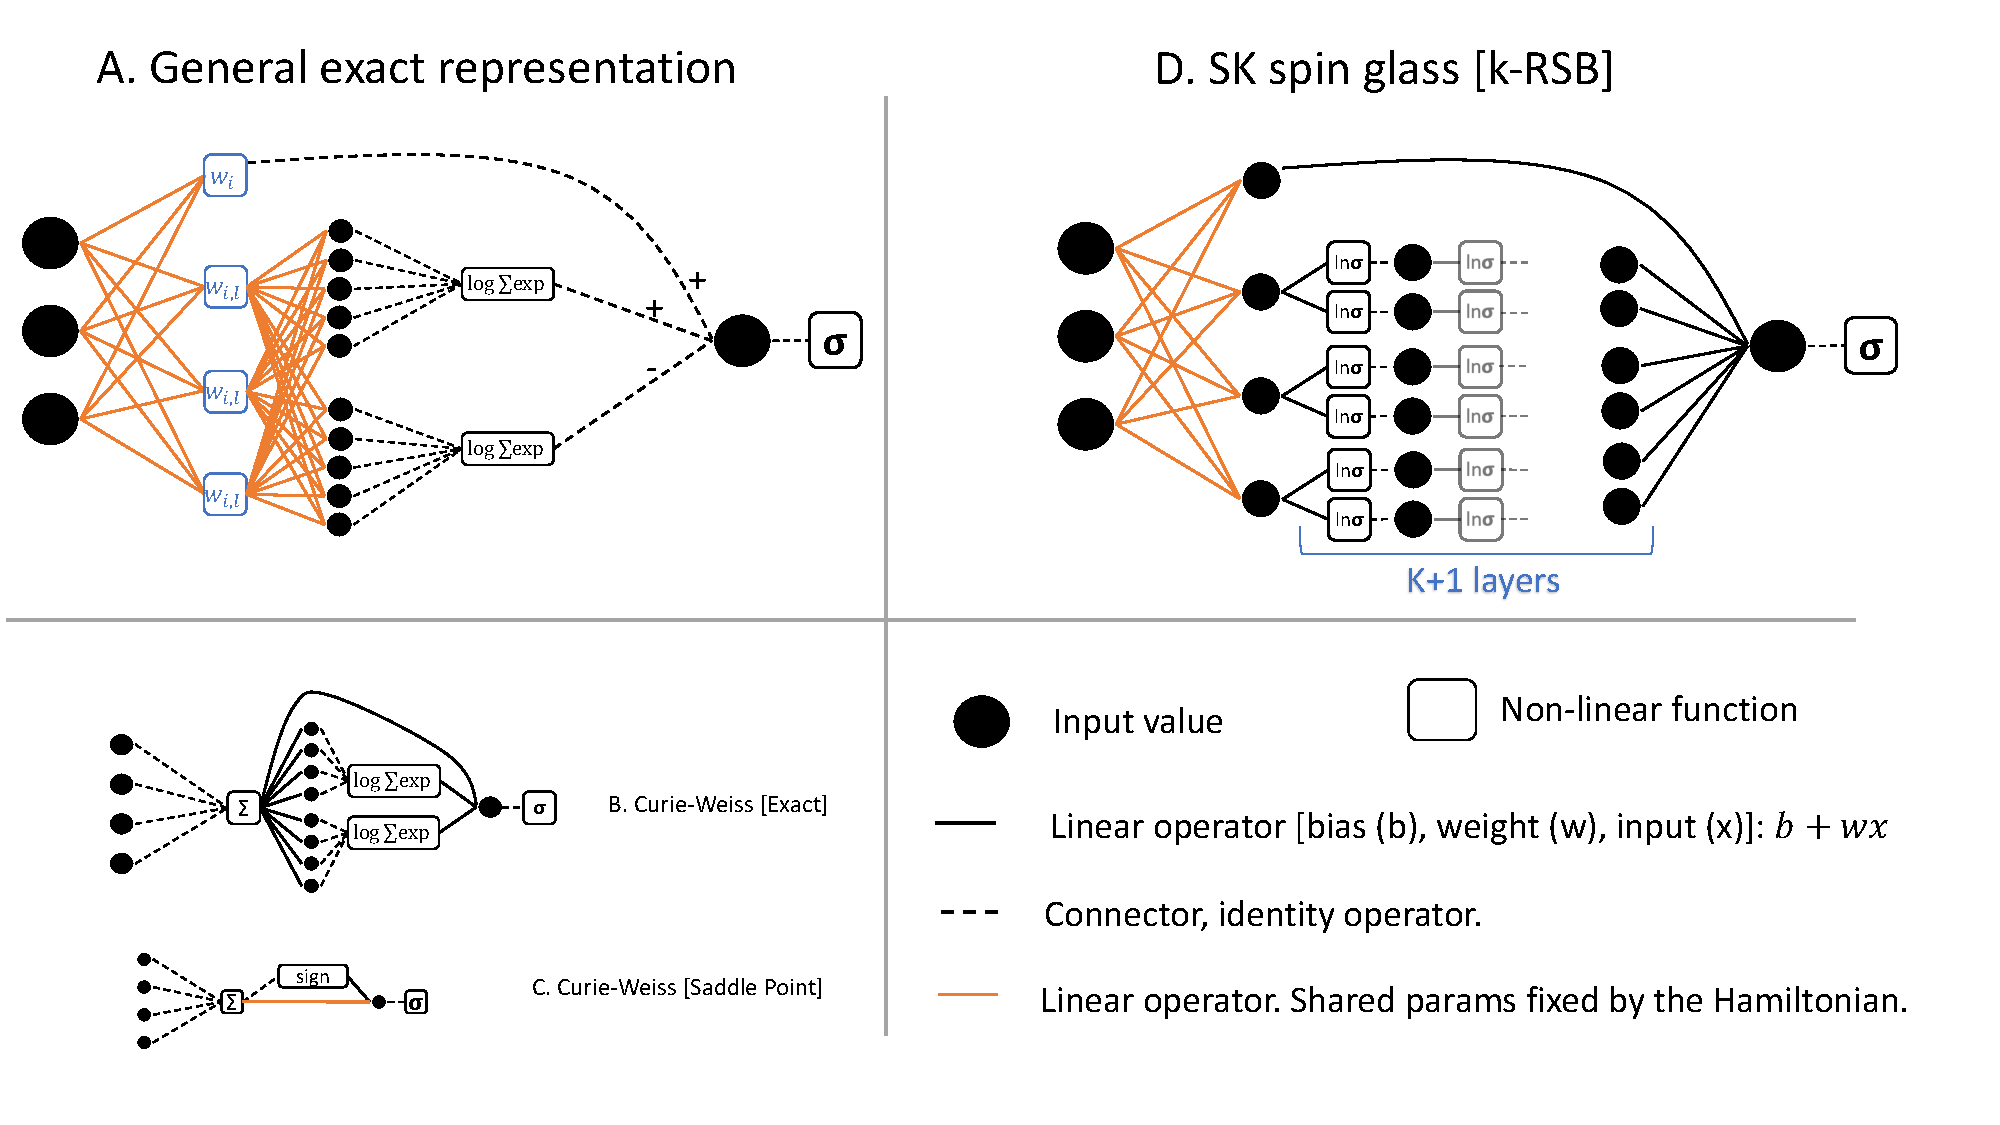
\includegraphics[width=1\textwidth]{img/ann_img.pdf}
    \caption{Neural network Architectures of conditional probability}
    \label{fig:arch}
\end{figure}

\subsubsection{The recurrent inner structure of the hamiltonian autoregressive neural network}
\label{sec:inner_recurrent}
Consider the first layer of the GHANN, see figure \ref{fig:arch}.a. The first layer is composed of the following set of linear operators on the input $\omega_i(\mathbf{x}_{<i})=\sum_{s=1}^{i-1} J_{si} x_s$ and $\omega_{il}=\sum_{s=1}^{i-1} J_{sl} x_s$ with $i<l<=N$. The set of $\omega_{il}$ can be rewritten in recursive form observing that:
\begin{equation}
\omega_{il} = \omega_{i-1,l} + J_{i-1,l} x_{i-1}
\end{equation}
The neurons $\omega_{il}$ in the first layer of each conditional probability in the GHANN architecture depend on the $\omega_{i-1,l}$ of the previous conditional probability, lighting up the recurrent nature of the GHANN architecture. \\
\subsection{Models}
\subsubsection{Curie-Weiss model}

The Curie-Weiss model is a uniform, fully-connected Ising model. Its Hamiltonian, with $N$ spins, is:

\begin{equation}
H\left(\mathbf{x}\right)=-h\sum_{i=1}^{N}x_{i}-\frac{J}{N}\sum_{i<j}x_{i}x_{j}
\doteq -h\sum_{i=1}^{N} S - \frac{J}{2N}S^2 + \frac{J}{2}
\end{equation}
 where we have defined $S=\sum_{i=1}^{N}x_{i}$.\\
 The conditional probability of a spin $i$ to be up, given the configuration of the other smaller spins $\mathbf{x}_{<i}$:
\begin{equation}
P\left(x_{i}=1|\mathbf{x}_{<i}\right) = \sigma\left( 
 2 \beta h + 2 \beta \frac{J}{N}\sum_{s=1}^{i-1}x_s +\log(\rho_i^+[\mathbf{x}_{<i}]) - \log(\rho_i^-[\mathbf{x}_{<i}])
\right),
\end{equation}
where:
\begin{equation*}
\rho_i^{\pm}[\mathbf{x}_{<i}] = \sum_{x_{i+1}\dots 
x_{N}}e^{\beta \left(h\pm\frac{J}{N}+\frac{J}{N}\sum_{s=1}^{i-1}x_{s}\right)S_{i}+\frac{\beta J}{2N}S_{i}^{2}} = 
\sum_{x_{i+1}\dots x_{N}} e^{\beta h_i^{\pm}[\mathbf{x}_{<i}]S_i +\frac{\beta J}{2N}S_{i}^{2}},
\end{equation*}
and we defined $h_i^{\pm}[\mathbf{x}_{<i}] = h\pm\frac{J}{N}+\frac{J}{N}\sum_{s=1}^{i-1}x_{s}$ and $S_i=\sum_{l=i+1}^{N}x_{l}$. The sums over the configurations of the spins $l$ can be carried on easily:
\begin{eqnarray*}
 \rho_i^{\pm}[\mathbf{x}_{<i}] & = & \sum_{x_{i+1}\dots x_{N}} e^{\beta h_i^{\pm}[\mathbf{x}_{<i}]S_i +\frac{\beta J}{2N}S_{i}^{2}}
  = \sqrt{\frac{N}{2\pi \beta J}}\sum_{x_{i+1}\dots x_{N}}e^{\beta h_i^{\pm}[\mathbf{x}_{<i}] S_{i}}\int e^{-\frac{N}{2J \beta}t^{2}+t S_{i}} dt\\
 & = & \sqrt{\frac{N}{2\pi \beta J}}\int dt e^{-\frac{N}{2J \beta}t^{2}} \sum_{x_{i+1}\dots x_{N}}e^{(\beta h_i^{\pm}[\mathbf{x}_{<i}] + t) S_{i}}  
 =  \sqrt{\frac{N}{2\pi \beta J}}\int dt e^{-\frac{N}{2J \beta}t^{2}} \left(e^{\beta h_i^{\pm}[\mathbf{x}_{<i}] + t} + e^{ (-\beta h_i^{\pm}[\mathbf{x}_{<i}] - t)} \right)^{N-i}  \\ 
 \label{eq:rho_last_exact}
 \end{eqnarray*} 
 whwre we used the Hubbard–Stratonovich (HS) transformation to get the second equality.\\
 First, in the following,  we derive the exact expression of the this conditional probability and how it can be expressed as a feed forward neural network, then the limit to $n\rightarrow N$ we derive a new architecture with smaller number of parameters.\\



 \subsubsection{Exact expression of the conditional probability of the Curie-Weiss model}
 The integral in the equation \ref{eq:rho_last_exact} can be computed the following way:

 \begin{eqnarray*}
 \rho_i^{\pm}[\mathbf{x}_{<i}] &=& \sqrt{\frac{N}{2\pi \beta J}}\int dt e^{-\frac{N}{2J \beta}t^{2}} 
 \sum_{k=0}^{N-i} \binom{N-i}{k} e^{(N-i-2k)*(\beta h_i^{\pm}[\mathbf{x}_{<i}] + t)}\\
 &=& \sum_{k=0}^{N-i} \binom{N-i}{k} \sqrt{\frac{N}{2\pi \beta J}}\int dt e^{-\frac{N}{2J \beta}t^{2}} 
  e^{(N-i-2k)*(\beta h_i^{\pm}[\mathbf{x}_{<i}] + t)}\\
&=& \sum_{k=0}^{N-i} \binom{N-i}{k}e^{\frac{\beta J}{2N}\left(N-i-2k\right)^{2}+\left(N-i-2k\right)\left(\beta h \pm \frac{\beta J}{N}\right)} e^{\frac{\beta J}{N}\left(N-i-2k\right) \sum_s x_s} \\
&=& \sum_{k=0}^{N-i} e^{a_{i,k}^{\pm} + b_{i,k}^{\pm} \sum_s x_s} 
\end{eqnarray*}
where we defined:
\begin{eqnarray}
\label{eq:params}
e^{b_{i,k}^{\pm}} & = & \binom{N-i}{k}e^{\frac{\beta J}{2N}\left(N-i-2k\right)^{2}+\left(N-i-2k\right)\left(\beta h \pm \frac{\beta J}{N}\right)}\\
e^{\omega_{i,k}^{\pm}} & = & e^{\frac{\beta J}{N}\left(N-i-2k\right)}.
\end{eqnarray}
The final feed-forward architecture of the neural network is:
\begin{eqnarray}\
\label{eq:curie_weiss_cond}
Q^{\Theta}\left(x_{i}=+1|\mathbf{x}_{<i}\right) & = &  \sigma \left(b_{i}+\omega_{i}\sum_{s=1}^{i-1}x_{s}-\log\left[\sum_{k=0}^{N-i}e^{b_{i,k}^{+}+w_{i,k}^{+}\sum_{s=1}^{i-1}x_{s}}\right]+\log\left[\sum_{k=0}^{N-i}e^{b_{i,k}^{-} + w_{i,k}^{-}\sum_{s=1}^{i-1}x_{s}}\right]\right).
\end{eqnarray}
where $b_i=2\beta h$ and $\omega_i=\frac{2\beta J}{N}$. 
\newline
This function can be interpreted as a feed-forward neural network; see fig.\ref{fig:curie_weiss}. 
The parameters of this neural network have an analytic dependence from the parameters $J$ and $h$ of the Boltzmann distributions. 
The set of parameters ($b_i, b_i^{k\pm}, \omega_i, \omega_i^{k\pm}$) can be consider as free parameters trained to minimize the KL divergence with the true probability distribution. 
It is interesting to note the number of parameters of each conditional probability distribution $i$ are $2+4(N-i)$; they decrease as $i$ increase as well as their number of variable in the input. This results is, somehow, the opposite on what usually the architecture should take care, meaning enlarging the number of input variables the number of parameters should increase as well to describe the complexity of the function to represent. Moreover the conditional probability neural network depends only of the sum of the input variables.
The total number of parameters of all conditional probability distribution scale as $O(N^2)$. 

\begin{figure}[!h]
    \centering
    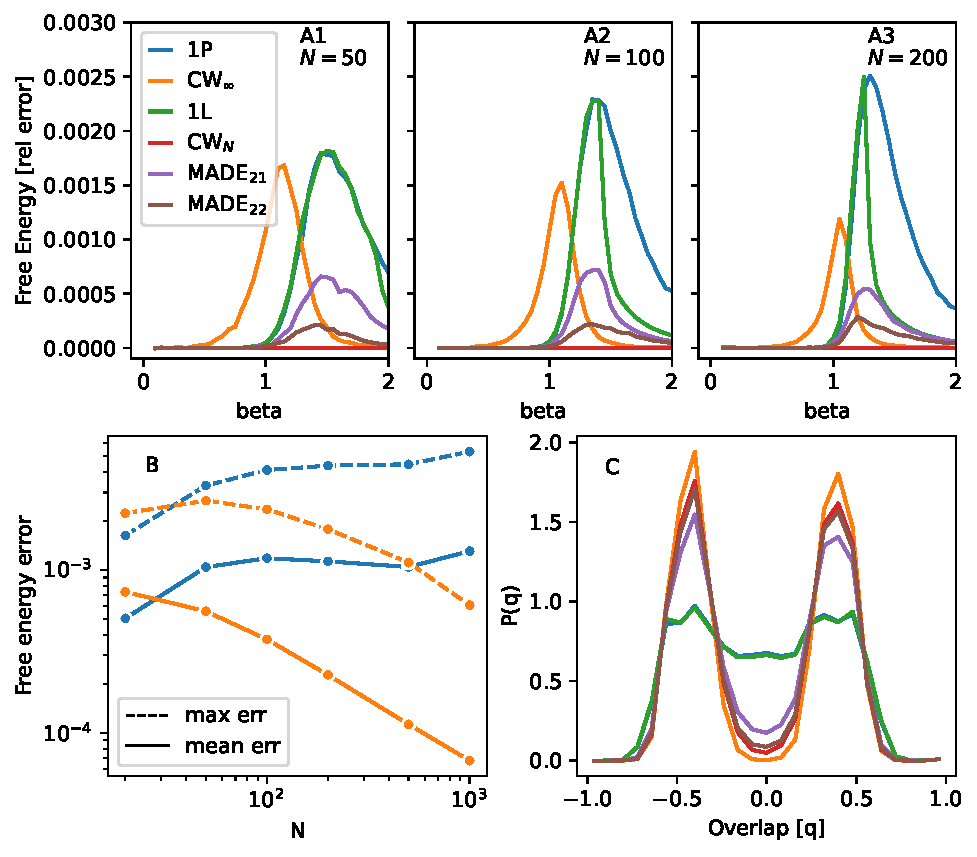
\includegraphics[width=1\textwidth]{img/CW_res.pdf}
    \caption{Results}
    \label{fig:curie_weiss}
\end{figure}


\subsubsection{Saddle point method}
Now we derive a new neural network architecture in the limit of $N \gg 1$. For simplicity the $h=0$ case is considered. Introducing the following variables: $\rho_i = \frac{N-i}{N}$, $m_i = -\frac{N-i-2k}{N}$, we can write:
 \begin{align*}
 \rho_i^{\pm}[\mathbf{x}_{<i}] &= \sqrt{\frac{N}{2\pi \beta J}}\int dt e^{-\frac{N}{2J \beta}t^{2}} 
 \sum_{k=0}^{N-i} \binom{N-i}{k} e^{(N-i-2k)*(\beta h_i^{\pm}[\mathbf{x}_{<i}] + t)}\\
 &= \sum_{k=0}^{N-i} \binom{N-i}{k}e^{\frac{\beta J}{2N}\left(N-i-2k\right)^{2}+\left(N-i-2k\right)\left(\pm\frac{\beta J}{N}\right)} e^{\frac{\beta J}{N}\left(N-i-2k\right) \sum_s x_s} \\
 &= \sum_{m_i=-\rho_i}^{\rho_i} \binom{N\rho_i}{\frac{N(m_i+\rho_i)}{2}} e^{\frac{N \beta J}{2}m_i^{2} \mp \beta J m_i } e^{N \rho_i \beta J \frac{\sum_s x_s}{N-i}}
\end{align*}
In the limit $N \gg 1$, and using the Stirling approximation for the binomial factor we obtain:
 \begin{align*}
 \rho_i^{\pm} &= 
  \int_{-\rho_i}^{\rho_i} \binom{N\rho_i}{\frac{N(m_i+\rho_i)}{2}} e^{\frac{N \beta J}{2}m_i^{2} \mp \beta J m_i } e^{N \rho_i \beta J \frac{\sum_s x_s}{N-i}} dm_i \\
& =  \int_{-\rho_i}^{\rho_i} \exp\left\{-N\rho\left( -\frac{1+\frac{m_i}{\rho_i}}{2} \log\frac{1+\frac{m_i}{\rho_i}}{2} - \frac{1-\frac{m_i}{\rho_i}}{2} \log\frac{1-\frac{m_i}{\rho_i}}{2}   - \frac{\beta m_i^2}{2 \rho_i} + \beta m_i \frac{\sum_s x_s}{N-i}\right) \right\} e^{\mp \beta J m_i}
\end{align*}
Now we use the saddle point method to evaluate this integrals, computing the extremes of the function inside the curly brackets. Deriving by $m_i$ we obtain that the extremes should satisfy the following equation:
\begin{equation}
\frac{m_i}{\rho_i} = \tanh \left( \beta(\frac{m_i}{\rho_i} - \frac{\sum_s x_s}{N-i}) \right)
\label{eq:extrem_i}
\end{equation}
In the $N$ large limit, and for a typical sample, we assume that: $\frac{\sum_s x_s}{N-i} \approx |\tilde{m}_{\beta}| \text{sign}(\sum_s x_s)$, where the $\tilde{m}_{\beta}$ is the magnetization of the Curie-Weiss system at inverse temperature $\beta$ and $\text{sign(x)} = \frac{|x|}{x}$ is the sign function.
We can distinguish two cases when the magnetization of the system is zero or different from zero. 
In the first case, when $\beta\leq1$, the solution of eq.\ref{eq:extrem_i} is zero as well, and $\log(\rho_i^{+}) - \log(\rho_i^{-})=0$ because the only term that depends on the sign, $\mp \beta J m_i$, vanish.\\ 
When instead the system acquire a magnetization $\tilde{m}_{\beta}$ different from zero, the eq.\ref{eq:extrem_i} admit one maximum, that depends on the two possible symmetric values of $\frac{\sum_s x_s}{N-i}\approx |\tilde{m}_{\beta}| \text{sign}(\sum_q x_q)$. 
The solution of eq.\ref{eq:extrem_i}, $\pm \tilde{m}_{\text{extrem}}$ depends again on $\text{sign}(\sum_s x_s)$. 
Once again we can write the maximum solution as $\tilde{m}_{i}=|\tilde{m}_i| \text{sign}(\sum_s x_s)$. 
Easily we obtain that $\log(\rho_i^{+}) - \log(\rho_i^{-}) = -2\beta J|\tilde{m}_i| \text{sign}(\sum_s x_s)$. 
We can use a trial function in this form:
\begin{eqnarray}\
\label{eq:curie_weiss_cond2}
Q^{\Theta}\left(x_{i}=+1|\mathbf{x}_{<i}\right) & = & \sigma \left(\omega_{i}^0\sum_{s=1}^{i-1}x_{s} + \omega_i^1 \text{sign}(\sum_{s=1}^{i-1}x_{s})\right).
\end{eqnarray}
where $\omega_i^{1,2}$ are free parameters to be trained. The number of parameters in this case scale as $O(N)$.

\section{spin glass}
Consider the hamiltonian of a spin glass with zero external field for simplicity:
\begin{equation}
H\left(\mathbf{x}\right)=-\sum_{i<j}J_{ij}x_{i}x_{j}
\end{equation}
where the set of $\underline{J}$ are i.i.d. random variable extracted from a Gaussian probability distribution $P(J)=\sqrt{\frac{N}{2\pi}}\exp\left(\frac{-NJ^2}{2} \right)$. \\
To find a feed-forward representation of the conditional probability of the Sherrington-Kirkpatrick model we use the replica trick \cite{}. We assume that $N-i$ is large enough such that the following approximation is valid for the partial partition function $\rho_i$: 
\[
\log\rho_i^{\pm} \sim \mathbb{E}\left[  \log\rho_i^{\pm} \right] = \lim_{n\rightarrow 0} \frac{  \log(\mathbb{E}\left[(\rho_i^{\pm})^n \right])}{n}
\]

Where in the last passage we use the replica trick. We assume that the quantity $\log\rho_i^{\pm}$ is a self-averaged quantity on the $N-i$ variables. The replica computation can be carried on easly, finding:
\begin{eqnarray}
\mathbb{E}_{\underline{J}}\left[(\rho_i^{\pm}[\mathbf{x}_{<i}])^n \right] & = & 
\int \prod_{l<l'} dP_{J_{ll'}} \left[ 
\sum_{\{\underline{x}^{a}\}_{i+1}^N} \exp\left\{\beta \left[
\sum_{l,a}\left( \pm J_{il} + \sum_{s} J_{sl} x_s \right) x_l^{a} + \sum_{l,l', a} J_{ll'} x_l^{a} x_{l'}^{a}
\right]  \right\} 
\right]\\
\end{eqnarray}
where, the sums over $(l,l')$, $s$ and $a$ run respectively over $(i+1,N)$, $(1,i-1)$ and $(1,n)$, and $dP_{J_{ll'}}=P(J_{ll'})dJ_{ll'}$. We defined $h_l^{\pm}[\mathbf{x}_{<i}] =\pm J_{il} + \sum_{s=1}^{i-1} J_{sl} x_s$ and carrying out the integrals over the disorder variables $\{P(J_{ll'})\}$ yields:
\begin{eqnarray}
\mathbb{E}_{\underline{J}}\left[(\rho_i^{\pm}[\mathbf{x}_{<i}])^n \right] & = & 
\sum_{\{\underline{x}^{a}\}_{i+1}^N} 
\exp\left\{\beta \left[
\sum_{l} h_l^{\pm}[\mathbf{x}_{<i}] \sum_{a} x_l^{a} +\frac{\beta}{2N} \sum_{l,l'} \sum_{a,b} x_l^{a} x_l^{b} x_{l'}^{a}x_{l'}^{b} \right]  \right\} \\
& = & e^{ \frac{(N-i) \beta^2}{4N}((N-i)n-n^2) } 
\sum_{\{\underline{x}^{a}\}_{i+1}^N} 
\exp\left\{\beta \left[
\sum_{l} h_l^{\pm}[\mathbf{x}_{<i}] \sum_{a} x_l^{a} +\frac{\beta}{2N} \sum_{a<b} \left( \sum_{l}  x_l^{a} x_l^{b} \right)^2 \right]  \right\}
\end{eqnarray}
Using the Hubbard-Stratonovich transformation of the quadratic terms we car write:
\begin{eqnarray}
\mathbb{E}_{\underline{J}}\left[(\rho_i^{\pm}[\mathbf{x}_{<i}])^n \right] & = & 
c(n,N,i)
\int \prod_{a<b} dQ_{ab} e^{-\frac{N}{2}\beta^2Q_{a,b}^2}
\sum_{\{\underline{x}^{a}\}_{i+1}^N} 
\exp\left\{\beta \left[
\sum_{l} h_l^{\pm}[\mathbf{x}_{<i}] \sum_{a} x_l^{a} +\beta \sum_{a<b} Q_{a,b} \sum_{l}  x_l^{a} x_l^{b} \right]  \right\} \\
& = & 
c(n,N,i)
\int \prod_{a<b} dQ_{ab} e^{-\frac{N}{2}\beta^2Q_{a,b}^2}
\prod_{l} \left[
\sum_{\{\underline{x}^{a}_l\}} 
\exp\left\{\beta \left[
h_l^{\pm}[\mathbf{x}_{<i}] \sum_{a} x_l^{a} +\beta \sum_{a<b} Q_{a,b}  x_l^{a} x_l^{b} \right]  \right\}
\right] \label{eq:before_ansaltz}
\end{eqnarray}
where we defined $c(n,N,i) = e^{ \frac{(N-i) \beta^2}{4N}((N-i)n-n^2) } \left(\frac{2\pi \beta^2}{N}\right)^{\frac{n(n-1)}{2}}$. The well know Parisi solutions of the SK model prescribe how to parametrize \cite{} the matrix of the overlaps $Q$. In the following we show how to obtain neural network architectures based on the the replica symmetric (RS) and k-replica symmetric broken symmetry (k-RSB) solutions.

\begin{figure}[!h]
    \centering 
    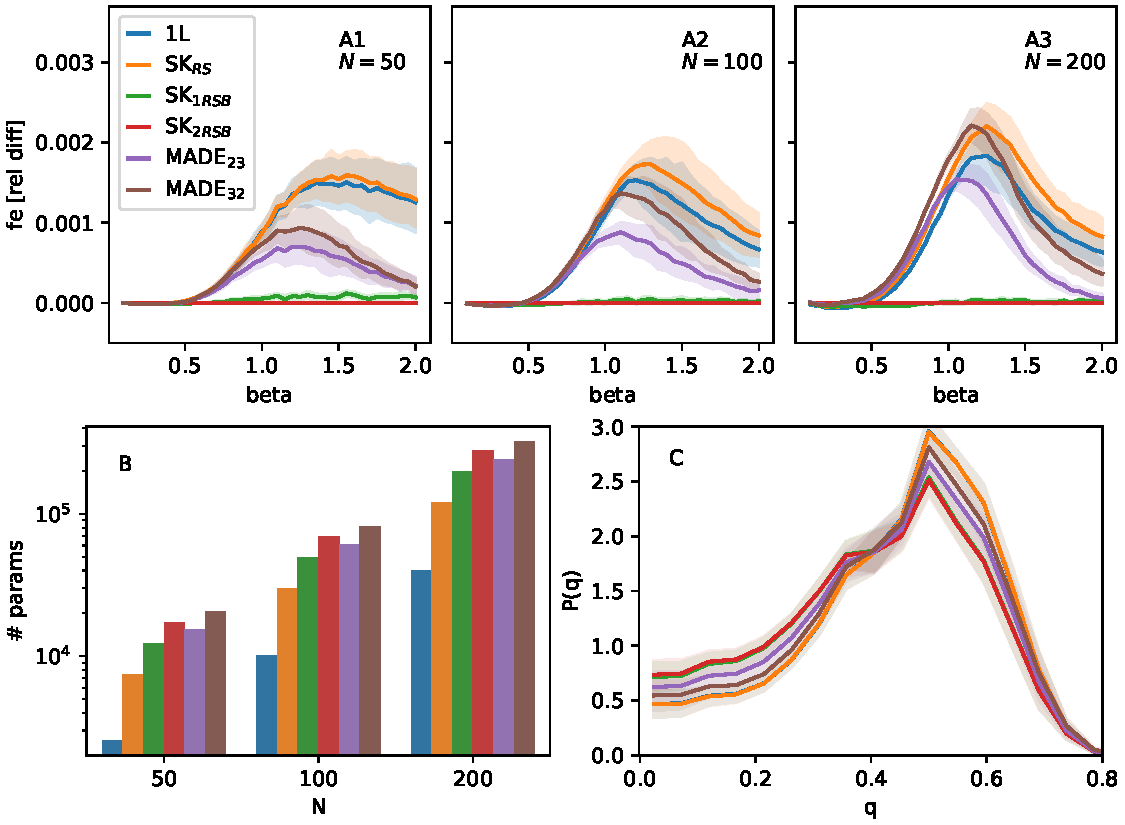
\includegraphics[width=1\textwidth]{img/SK_res.pdf}
    \caption{Results}
    \label{fig:curie_weiss}
\end{figure}


\subsection{Replica Symmetric solution (RS)}
We assume that the overlap between the replicas symmetric under permutations, and the matrix of the overlaps between replicas is parametrize with only one variable $q$:
$$
Q_{a,b}=\begin{cases}
			0, & \text{if $a=b$}\\
            q, & \text{otherwise}
		 \end{cases}
$$
Considering this ansatz we obtain:
\begin{eqnarray}
\mathbb{E}_{\underline{J}}\left[(\rho_i^{\pm, sym}[\mathbf{x}_{<i}])^n \right] & = & 
c(n,N,i)
\int dq e^{-\frac{n(n-1)N}{4}\beta^2 q^2}
\prod_{l} \left[
\sum_{\{\underline{x}^{a}_l\}} 
\exp\left\{\beta \left[
h_l^{\pm}[\mathbf{x}_{<i}] \sum_{a} x_l^{a} +\beta q \sum_{a<b} x_l^{a} x_l^{b} \right]  \right\} 
\right] \\
& = &
c(n,N,i)
\int dq e^{-\frac{n(n-1)N}{4}\beta^2 q^2}
e^{-\frac{nN\beta^2 q}{2}}
\prod_{l} \left[
\sum_{\{\underline{x}^{a}_l\}} 
e^{\beta \left[
h_l^{\pm}[\mathbf{x}_{<i}] \sum_{a} x_l^{a} + \frac{\beta q}{2} \left(\sum_{a} x_l^{a} \right)^2 \right]} 
\right]\\
& = &
c'(n,N,i)
\int dq e^{-\frac{n(n-1)N}{4}\beta^2 q^2}
e^{-\frac{nN\beta^2 q}{2}}
\prod_{l} \left[\int \frac{dz_l}{\sqrt{2\pi q}} e^{-\frac{z_l^2}{q}}
\sum_{\{\underline{x}^{a}_l\}} 
e^{\beta \left(
h_l^{\pm}[\mathbf{x}_{<i}] +\beta z_l \right) \sum_{a} x_l^{a}} 
\right]\\
& = &
c'(n,N,i)
\int dq e^{-nN\left(\frac{(n-1)}{4}\beta^2 q^2 +\frac{\beta^2 q}{2}\right)}
\prod_{l} \left[\int \frac{dz_l}{\sqrt{2\pi q}} e^{-\frac{z_l^2}{q}}
2^n\cosh^n \left(\beta \left(
h_l^{\pm}[\mathbf{x}_{<i}] +\beta z_l \right)\right) 
\right].\\
\end{eqnarray}
Using the limit that $n\rightarrow 0$ we can write:
\begin{eqnarray}
\int \frac{dz_l}{\sqrt{2\pi q}} e^{-\frac{z_l^2}{q}}
2^n\cosh^n \left(\beta \left(
h_l^{\pm}[\mathbf{x}_{<i}] +\beta z_l \right)\right) = e^{n \int \frac{dz_l}{\sqrt{2\pi q}} e^{-\frac{z_l^2}{q}}
\log 2\cosh \left(\beta \left(
h_l^{\pm}[\mathbf{x}_{<i}] +\beta z_l \right)\right)}.
\label{eq:gauss_n0}
\end{eqnarray}
And in the end we have:
\begin{eqnarray}
\log (\rho_i^{\pm, sym}[\mathbf{x}_{<i}]) & = & 
\lim_{n\rightarrow 0} \frac{1}{n} \log \left( c'(n,N,i)
\int dq e^{-\frac{n(n-1)N}{4}\beta^2 q^2}
e^{-\frac{nN\beta^2 q}{2}}
e^{n \sum_l 
\int \frac{dz_l}{\sqrt{2\pi q}} e^{-\frac{z_l^2}{q}}
\log 2\cosh \left(\beta \left(
h_l^{\pm}[\mathbf{x}_{<i}] +\beta z_l \right)\right)
} 
\right)\\
& = &
\log(c''(N,i)) + 
\left( +\frac{N}{4}\beta^2 q^2_0 
-\frac{N\beta^2 q_0}{2}
+ \sum_l 
\int \frac{dz_l}{\sqrt{2\pi q_0}} e^{-\frac{z_l^2}{q_0}}
\log 2\cosh \left(\beta \left(
h_l^{\pm}[\mathbf{x}_{<i}] +\beta z_l \right)\right)
\right) \\
& \doteq &  
c(N,i, q_0) -
\sum_l 
\int \frac{dz_l}{\sqrt{2\pi q_0}} e^{-\frac{z_l^2}{q_0}}
\log \sigma \left(\beta \left(
2h_l^{\pm}[\mathbf{x}_{<i}] +2\beta z_l \right)\right)
 \\
\end{eqnarray}
In the second line we use the saddle point methods to evaluate the integral over $q$, assuming tha the single maximum value $q_0$ doesn't depend from the input values $\mathbf{x}_{<i}$ in the set of $h_l^{\pm}[\mathbf{x}_{<i}]$. It is a strong assumption to be verified {\it a posteriori} on the goodness of the neural network architectures performances. In the third lines we simplify values that are the same between $\log(\rho^+)$ and $\log(\rho^-)$.

% We can, after some manipulations, obtain a more neural network friendly function:
% \begin{eqnarray}
% \log (\rho_i^{\pm, sym} [\underline{x_l}])^n] & \approx & 
% \text{Extr}_q \left( +\frac{N}{4}\beta^2 q^2 
% -\frac{N\beta^2 q}{2}
% + \sum_l 
% \int dz_l e^{-z_l^2}
% \log \cosh \left(\beta \left(
% h_l +\beta \sqrt{q}z_l \right)\right)
% \right) 
% \end{eqnarray}
Now we consider the following approximation of the following Gaussian convolution:
\[
\int dz e^{-z^2}
\log \sigma \left(\beta \left(
h +\beta \sqrt{q}z \right)\right) \sim b_0 + w_0*\log \sigma(b_1 + w_1 h) 
\]
Where $(b_0, w_0, b_1,w_1)$ are free parameters to be determined. In SI \cite{} a numerical analysis of the correctness of this approximation is shown.  
Putting together all the pieces we can parameterize the conditional probability as:
\begin{eqnarray}
Q^{RS}\left(x_{i}=1|\mathbf{x}_{<i}\right) & = & \sigma\left( 
-2 \beta H_{s}[x_i = +1] +\log(\rho_i^+) - \log(\rho_i^-)
\right) \\
& = & b_0^i + w_0^i\sum_q J_{si} x_{si} + \sum_{t \in \{+,-\}} w_0^{i,t} \sum_l \log\sigma(b_1^{i,t} + w_1^{i,t}\sum_{s} J_{sl} x_s) 
\end{eqnarray}
where the set of $(b,w)$ are free variational parameters to learn. The $\sum_t$ are the combinations of the plus and minus $\rho$ cases. 
\\DO the image of the nets.


\subsection{Finite Replica symmetric breaking (k-RSB)}
Assuming that the replica symmetry is broken we can use the following ansatz called 1 replica symmetric breaking (1RSB), where the overlaps between replicas are divided in $m$ blocks:
\begin{eqnarray}
    Q_{a,b}=\begin{cases}
			q_1, & \text{if $I(a/m)=I(b/m)$}\\
            q_0. & \text{if I(a/m) $\neq$ I(b/m)}
		 \end{cases}
\end{eqnarray}
With the above ansatz we can compute the following quantities:
\begin{eqnarray}
\sum_{ab} Q_{ab} x_{a} x_{b} &=& \frac{1}{2} \left[ q_0 \left( \sum_{a}x_a\right)^2 + (q_1-q_0) \sum_{\text{blocks}} \left( \sum_{a \in \text{block}}x_a\right)^2  -nq_1\right] \\
\sum_{ab} Q_{ab}^2 &=&  n^2 q_0^2 + nm(q_1^2 - q_0^2) -n q_1^2.
\end{eqnarray}
The equation \ref{eq:before_ansaltz} becomes:
\begin{align}
\mathbb{E}_{\underline{J}} \left[(\rho_i^{\pm, 1RSB})^n \right] &=&  \\[1ex]
\begin{split}
& = c(n,N,i) \int dq_1 dq_0 e^{\frac{N}{2}\beta\left[n^2 q_0^2 + nm(q_1^2 - q_0^2) -n q_1^2\right]} 
\prod_{l} \biggl[ \sum_{\{\underline{x}^{a}_l\}} \exp\biggl\{\beta \bigl[ \\ 
 & \qquad h_l^{\pm} \sum_{a} x_l^{a} +q_0 \left( \sum_{a} x_p^{a} \right)^2 + (q_1-q_0) \sum_{\text{blocks}} \left( \sum_{a \in \text{block}}x_l^{a}\right)^2  -nq_1 \bigl]  \biggr\}  \biggr] 
\end{split}\\ 
\begin{split}
& = c(n,N,i) \int dq_1 dq_0 e^{\frac{N}{2}\beta\left[n^2 q_0^2 + nm(q_1^2 - q_0^2) -n q_1^2 -n q_1\right]} 
\prod_{l} \biggl[ \sum_{\{\underline{x}^{a}_l\}} \int dP_{z_l} \prod_{k=1}^{n/m} \int dP{y_{lk}} \\ 
 &  \qquad  \exp\biggl\{\beta \bigl[h_l^{\pm} \sum_{a} x_l^{a} +  z_l \sum_{a}x_l^{a} + \sum_{\text{blocks}}  y_{lk} \sum_{a \in \text{block}}x_l^{a}\bigl]  \biggr\}  \biggr] 
\end{split}\\ 
\begin{split}
& = c(n,N,i) \int dq_1 dq_0 e^{\frac{N}{2}\beta\left[n^2 q_0^2 + nm(q_1^2 - q_0^2) -n q_1^2 -n q_1\right]} 
\prod_{l} \biggl[ \int dP_{z_l}  \prod_{k=1}^{n/m} \int dP_{y_{lk}}\\ 
 &  \qquad  \cosh^m\biggl(\beta \bigl[h_l^{\pm}+  z_l +y_{lk}\bigl]  \biggr)  \biggr]
\end{split}\\ 
\begin{split}
& = c'(n,N,i) + c(n,N,i) \int dq_1 dq_0 e^{\frac{N}{2}\beta\left[n^2 q_0^2 + nm(q_1^2 - q_0^2) -n q_1^2 -n q_1\right]} 
\prod_{p} \int dP_{z_l}  \exp \biggl\{ \frac{n}{m} \log \biggl( \int dP_{y_{l}}\\ 
 &  \qquad  \cosh^m\biggl(\beta \bigl[h_l^{\pm}+ z_l + y_{l}\bigl]  \biggr)  \biggr) \biggr\}
\end{split}\\ 
\end{align}
where we defined:
\begin{align}
    dP_{z_l} & = \frac{dz_l}{\sqrt{2\pi q_0}}e^{\frac{z^2}{2q_0}}\\
    dP_{y_{lk}} & = \frac{dy_{lk}}{\sqrt{2\pi (q_1-q_0)}}e^{\frac{y_{lk}^2}{2 (q_i-q_0)}}
\end{align}
Considering $N \gg 1$ and $n\rightarrow 0$ to use the saddle point methods and the identity in eq.\ref{eq:gauss_n0}, we can write:
\begin{align}
\log (\rho_i^{\pm, 1RSB}) & = 
\lim_{n\rightarrow 0} \frac{1}{n} \log \left(\mathbb{E}_{\underline{J}} \left[(\rho_i^{\pm, 1RSB})^n \right]  \right) \\
& = c_i +  \text{Extr}_{q_0, q_1} \biggl[ c'_i(N,n,q_0, q_1) 
+ \frac{1}{m} \sum_{l} \int dP_{z_l} \log \biggl( \int dP_{y_{l}} \cosh^m\biggl(\beta \bigl[h_l^{\pm}+ z_l + y_{l}\bigl]  \biggr)  \biggr)
\biggr]
\end{align}
The above integrals are computed in approximate way as in the following:
\begin{align}
& \int dP_{z_l} \log \biggl( \int dP_{y_{l}}  \cosh^m\biggl(\beta \bigl[h_l^{\pm}+ z_l +  y_{l}\bigl]  \biggr)  \biggr) 
 = \\
& \int dP_{z_l} \log \biggl( \int dP_{y_{l}} e^{ m \log \cosh \left(\beta \left[h_l^{\pm}+  z_l +  y_{l}\right]  \right) } \biggr) 
 = \\
& \beta h_{l}^{\pm} + \int dP_{z_l} \log \biggl( \int dP_{y_{l}} e^{ y_{l} - m \log \sigma \left(\beta \left[h_l^{\pm}+ z_l + y_{l}\right]  \right) } \biggr) 
\end{align}
We have two nested gaussian convolution. In order to make more easy to compute this non-linear operator we are going to use a sequence of approximation similar to those used previously for RS case. Recalling $h_l^{\pm}[\mathbf{x}_{<i}] =\pm J_{il} + \sum_{s} J_{sl} x_s$, we consider the approximation of the nested gaussian convolution:
\begin{align}
f(\mathbf{x}_{<i}) = \int \frac{dz_l}{\sqrt{2\pi q_0}}e^{\frac{z^2}{2q_0}} \log \biggl( \int \frac{dy_{l}}{\sqrt{2\pi (q_1-q_0)}}e^{\frac{y_{l}^2}{2 (q_i-q_0)}} e^{ y_{l} - m \log \sigma \left(\beta \left[\pm J_{il} + \sum_{s} J_{sl} x_s + h + z_l + y_{l}\right]  \right) } \biggr) 
\end{align}
Fixed the parameters of the model $(\{J_{pq}\}, h, \beta)$, this is a function that depends from three free parameters $(q_0, q_1, m)$. I approximate the integrals with a feed forward scheme, enlarging the number of free parameters in order to have a feed forward function without integrals. First we consider the following maps:
\begin{align}
    \int dx e^{\frac{x^2}{a} + x + b \log\sigma (h + x)} &\approx a_0 (1 + e^{a_1 + b_1 \log \sigma (a_2 + b_2 h) }) = a_0 \sigma^{-1}(a_1 + b_1 \log \sigma (a_2 + b_2 h) )\\
    \int dx e^{\frac{x^2}{a}} \log\sigma (a_1 + b_1 \log \sigma (a_2 + b_2 (h+x))) &\approx a_0 +b_0 \log \sigma (a'_1 + b'_1 \log \sigma (a'_2 + b'_2 (h))) 
\end{align}
where the set of parameters $(a_0, a_1, a_2, b_1, b_2)$ are free parameters to be determined by the learning procedures. The for the 1RSB we use the following architecture:
\begin{eqnarray}
    Q^{1RSB}\left(x_{i}=1|\mathbf{x}_{<i}\right) & = & \sigma\left( 
    -2 \beta H_{s}[x_i = +1] +\log(\rho_i^+) - \log(\rho_i^-)
    \right) \\
    & = & b_0^i + w_0^i\sum_q J_{si} x_{si} + \sum_{t \in \{+,-\}} w_0^{i,t} \sum_l \log\sigma(b_1^{i,t} + w_1^{i,t}\log\sigma(b_2^{i,t} + w_2^{i,t}\sum_{s} J_{sl} x_s))
    \end{eqnarray}
The genralization of the above procedure for K-RSB is straightforward. For instance for 2-RSB we have:
\begin{eqnarray}
    &Q^{2RSB}\left(x_{i}=1|\mathbf{x}_{<i}\right)  =  \sigma\left( 
    -2 \beta H_{s}[x_i = +1] +\log(\rho_i^+) - \log(\rho_i^-)
    \right) \\
    & =  b_0^i + w_0^i\sum_q J_{si} x_{si} + \sum_{t \in \{+,-\}} w_0^{i,t} \sum_l \log\sigma(b_1^{i,t} + w_1^{i,t}\log\sigma(b_2^{i,t} + w_2^{i,t}\log\sigma(b_3^{i,t} + w_3^{i,t}\sum_{s} J_{sl} x_s))) 
    \end{eqnarray}

\section{Numerical evidence of Gaussian convolution approximations}
\paragraph{Curie Weiss model}
we have made the following approximation for representing the Curie-Weiss model in autoregressive form using the saddle point methods:
\[
\log \int dt e^{N(-\frac{t^2}{2K}+\log\cosh(K*h+t))} \approx \log\left(\sum_{t \in \text{Extrem}^+}  e^{b_i^t + c_i^t\log\cosh(d_i^t+e_i^t h)}\right)
\label{eq:CW_gauss_approx}
\]
\begin{figure}[h]
    \centering
    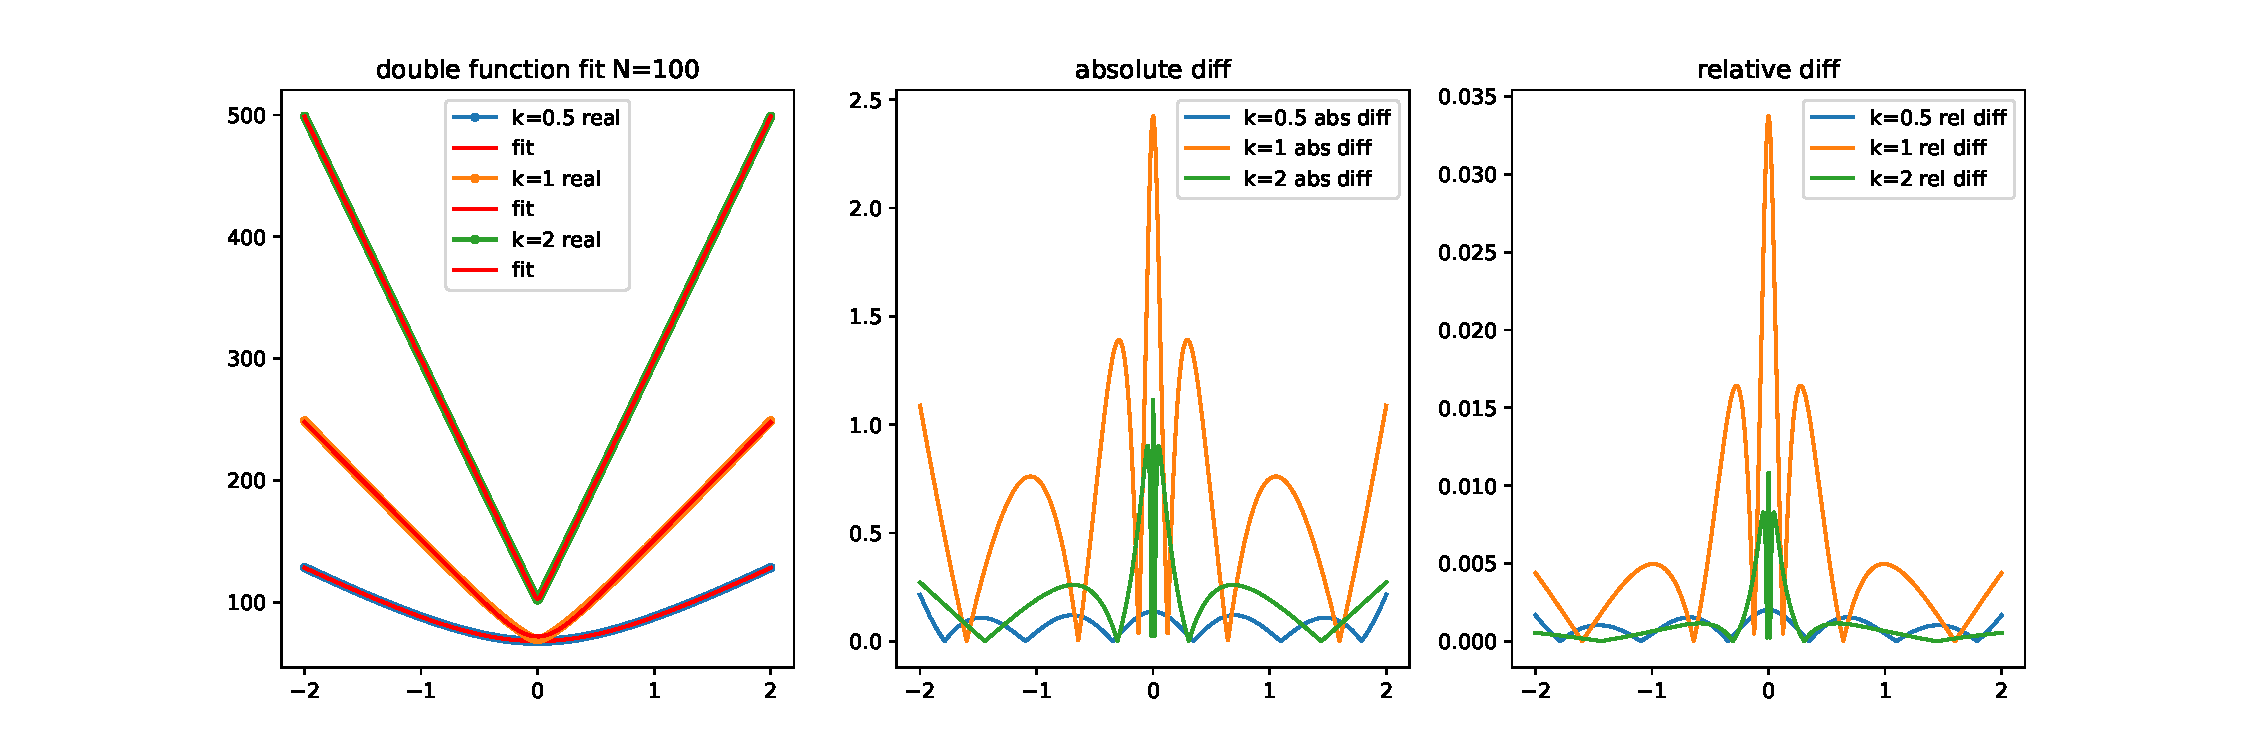
\includegraphics[width=1\textwidth]{img/CW_fit_N100.pdf}
    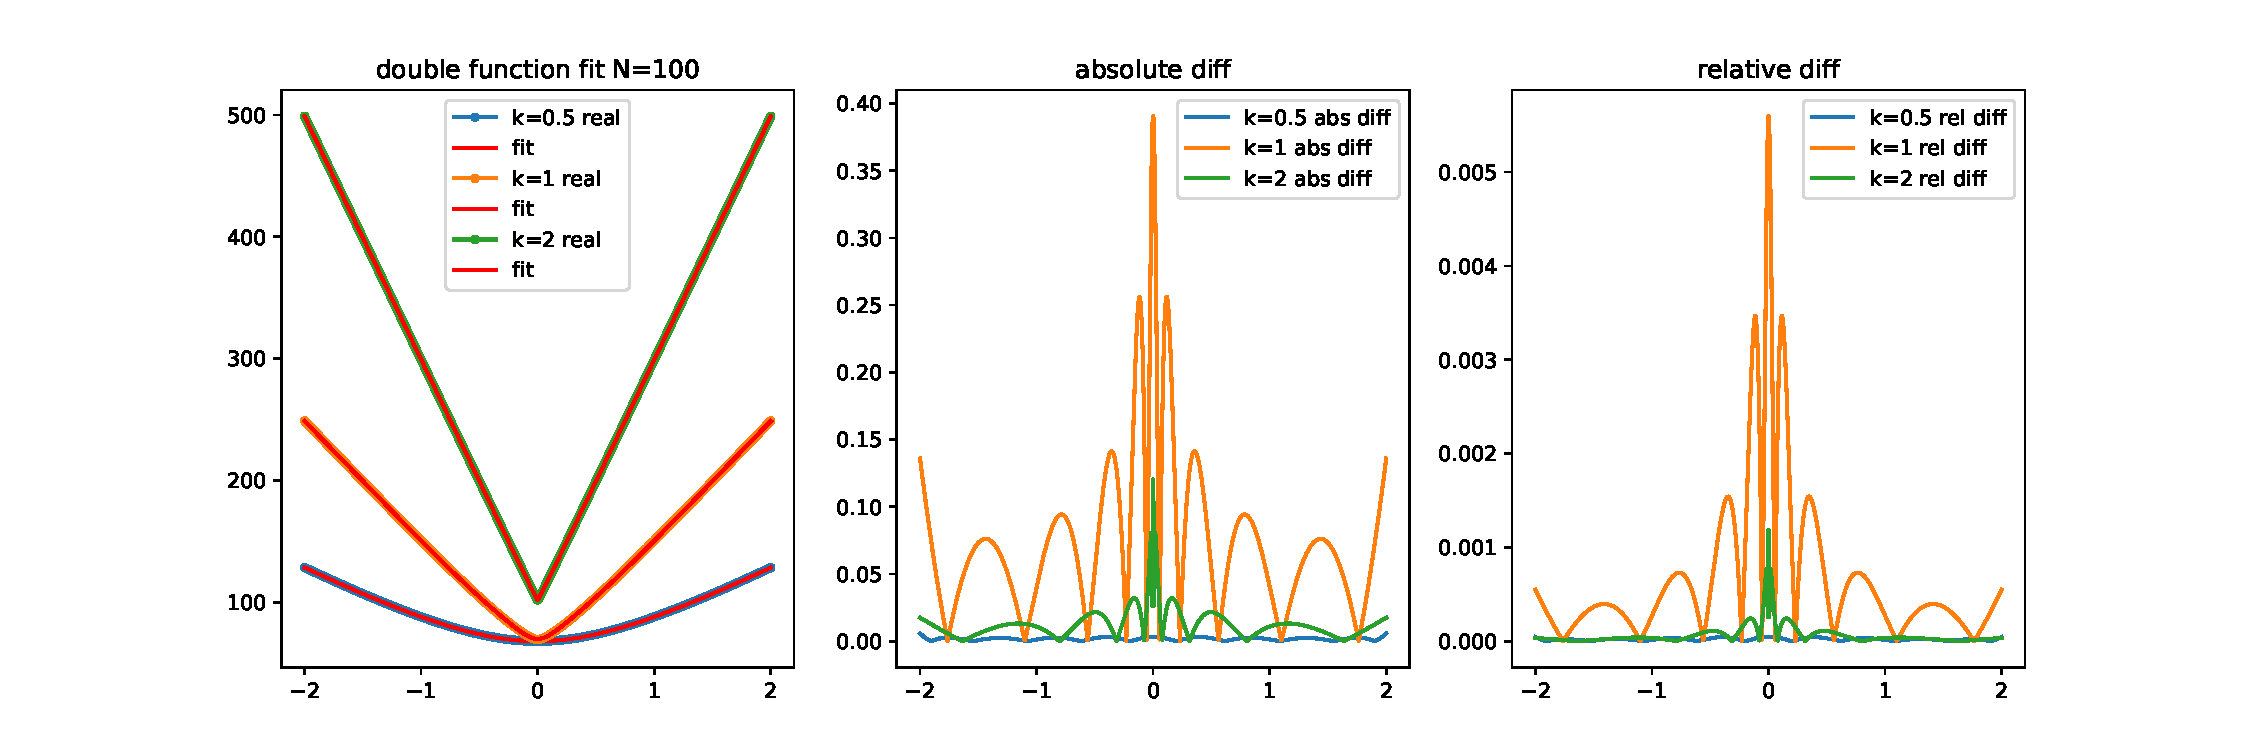
\includegraphics[width=1\textwidth]{img/CW_fit2_N100.pdf}
    \caption{Fit of eq.\ref{eq:CW_gauss_approx} at different values of $K=J\beta$. In the first row only one extreme is considered and two in the second row.}
    \label{fig:mesh1}
\end{figure}
The case of replica:
\[
 \int dt e^{-\frac{Nt^2}{2K}}\log\cosh(K*h+t) \approx \left(\sum_{t \in \text{Extrem}^+}  b_i^t + c_i^t\log\cosh(d_i^t+e_i^t h)\right)
\label{eq:CW_gauss_approx2}
\]

\begin{figure}[h]
    \centering
    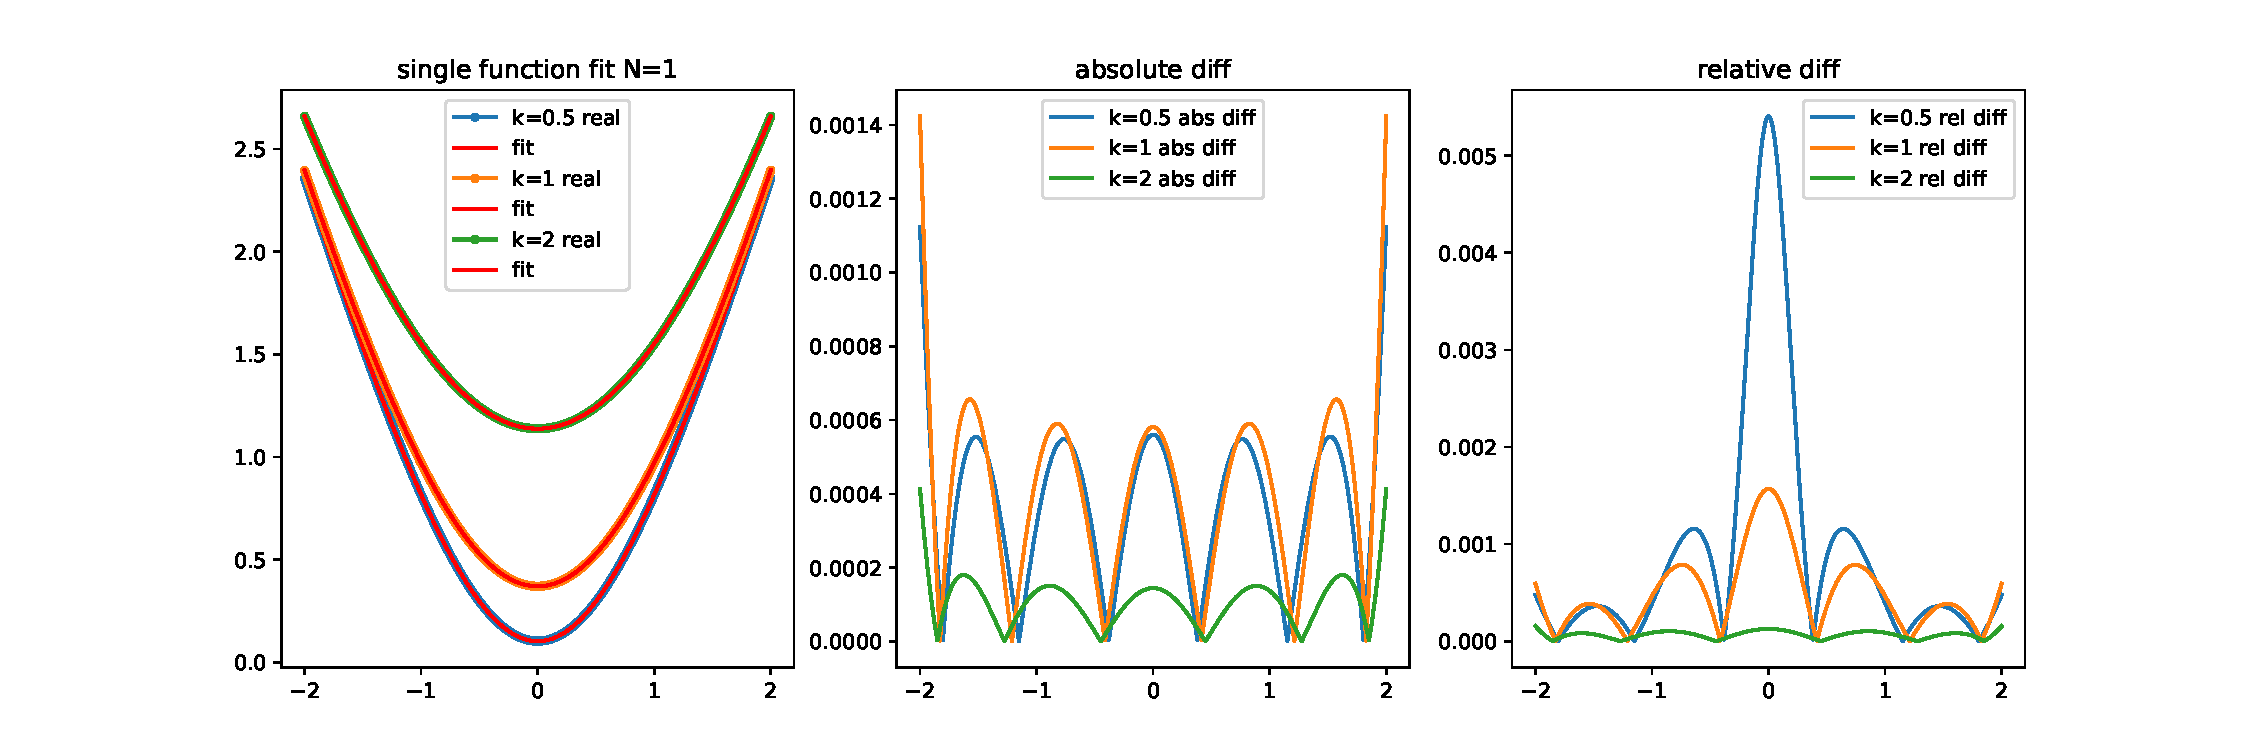
\includegraphics[width=1\textwidth]{img/RFIM_fit.pdf}
    \caption{Fit of eq.\ref{eq:CW_gauss_approx} at different values of $K=J\beta$. In the first row only one extreme is considered and two in the second row.}
    \label{fig:gauss_approx}
\end{figure}
\end{document}
  